\documentclass{article}
\usepackage{graphicx} 
\usepackage{tabularx}
\usepackage{lscape}
\usepackage{colortbl}
\usepackage[dutch]{babel}
\begin{document}
\sffamily
\begin{titlepage}
  \centering
    \vfill
    {\bfseries\Huge
      PVA Automated Systems, \\
      Project codename Beezkneez
        \vskip2cm
      }
      {\bfseries\Large
        Mark Steijger\\
      }
      {
        \bfseries\normalsize
        0938713\\
            \vskip1cm
    }
          {\bfseries\Large
        Kazimir Piek\\
      }
      {
        \bfseries\normalsize
        0953725\\
            \vskip1cm
    }      {\bfseries\Large
        Robert Karajev\\
      }
      {
        \bfseries\normalsize
        0851997\\
            \vskip1cm
    }      {\bfseries\Large
        Michael Francis\\
      }
      {
        \bfseries\normalsize
        0963038\\
            \vskip1cm
    }
            \vskip1cm
        \today\\
    \vfill
    
\includegraphics[width=4cm]{../IMAGES/logohr.png} % also works with logo.pdf
    \vfill
    \vfill
\end{titlepage}
\newpage
\tableofcontents

\newpage
\section{Inleiding}
Dit document dient als een techniesch naslagwerk voor AutomatedBeezzzz project, hierin worden de verschillende aspecten
die nodig zijn geweest voor het uiteindelijk complete product besproken. \cite{akbari_mohammadi_ziarati_2010}

\section{System/Subsystem Specification}
\section{System/Subsystem Design Description}



\subsection{System wide design decisions}
In dit hoofdstuk worden, zoals de tital al verraad, de design decisions behandeld. Hieronder vallen bijvoorbeeld
input/outputs van het systeem, gedrag keuzes en andere onderdelen die voor het gehele systeem gelden


\subsubsection*{Camera}
Aangezien het project inhoudt dat een aantal bijen gesimuleerd wordt, is het nodig om hun zintuigen ook te simuleren. Dit gebeurt door middel van een camera aan een raspberry pi. Hier zullen uiteraard eisen aan zitten, maar zullen in de SRS vermeldt worden. Om deze camera draadloos te laten werken is er ook een batterij pack nodig.

\subsubsection*{Server}
asd
\newline

\subsubsection*{Simulatie}
    \begin{center}
    \hspace*{-3.5cm}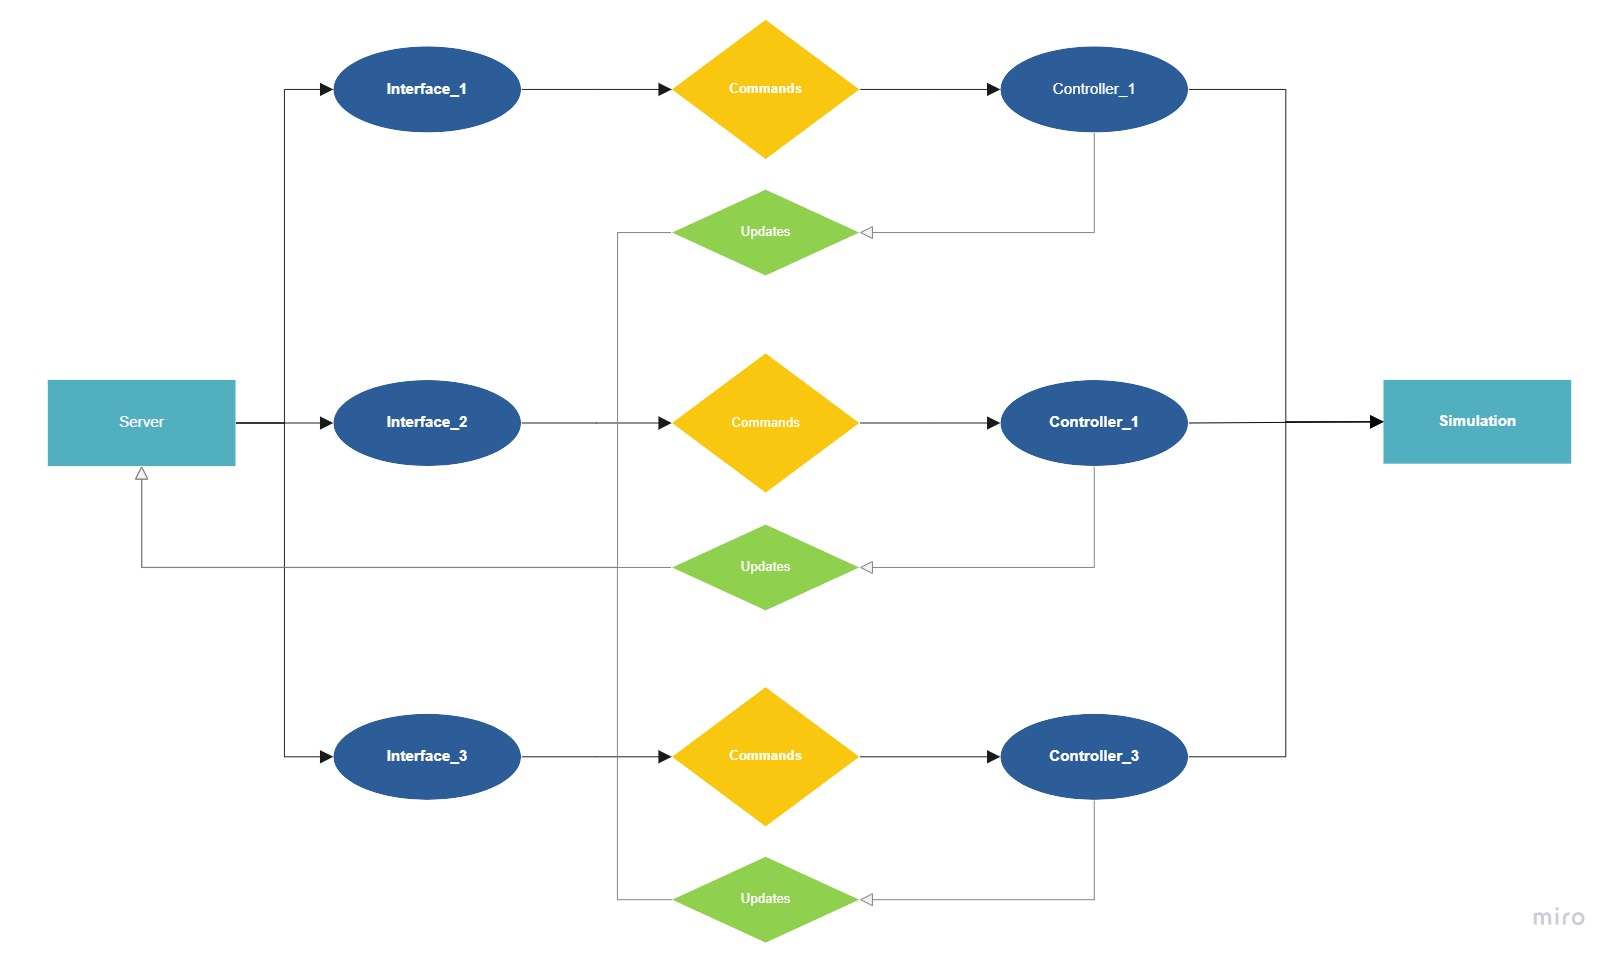
\includegraphics[width=1.6\textwidth]{../IMAGES/Simulation Interaction.jpg}
    \end{center}
    Het diagram hierboven weergeeft de communicatie tussen de simulatie en de server. In de simulatie
    wordt het gedrag van bijen met behulp van 3 ontworpen drones gesimuleerd. Om dat mogelijk te maken
    zijn voor de input en de output de volgende ontwerp keuzes gemaakt: \\

    \begin{description}\setlength{\itemindent}{0.1cm}
        \item[INPUT:] \hfill
        \begin{enumerate}
            \item De input voor de simulatie is altijd een opdracht naar een controller. Deze opdracht is een
            actie die een drone moet uitvoeren waarbij een positie meegegeven wordt  naarr de volgende verplaatsingsstap.
            Dit wordt mogelijk gemaakt door te communiceren tegen een opgebouwde interface. Deze
            interface communiceerd dan vervolgens tegen een controller die een gesimuleerde drone bestuurd.
        \end{enumerate}
        \newpage
        \item[OUTPUT:] \hfill
        \begin{enumerate}
            \item De output bij deze simulatie is verplaatsing van de gesimuleerde drone naar een geplannde positie.
            \item Daarnaast is er ook een andere continue output van de simulatie. Dat is een bericht die afkomstig
            is van een controller. Een controller stuurt om de bepaalde tijd een bericht naar de server met
            de informatie over de positie van de bestuurde drone.
        \end{enumerate}


    \end{description}

    \newpage
\subsection{System architectural design}
Uiteraard is het project een samenhangend geheel. Dit betekent dat er onderdelen zijn die afhankelijk zijn van andere onderdelen. Deze onderdelen zullen vermeld worden.

\subsubsection*{System components}
Diagram met hardware en software componenten van het gehelen systeem en de relatie tussen deze onderdelen < goeie, moeten we doen

Zoals op de afbeelding gebeeld wordt, is de camera afhankelijk van een raspberry pi. Dit komt omdat de beeld verwerkt moet worden door een microprocessor. Zo is er ook een samenhang tussen ...

% \section{Software Design Description}
\section{Software Requirement Specification}
In dit hoofdstuk word een opsomming en uitbreiding gegeven van de systeem requirements. Hieronder vallen onder andere
de modus/states waarin het systeem zich kan bevinden en de communicatie die plaatsvind om het systeem te laten werken.

\subsection{Requirements}

\subsubsection*{Camera}
Aan de camera zit een aantal eisen. Het meest voor de hand liggende eis is dat de resolutie hoog genoeg moet zijn
om bepaalde objecten te kunnen herkennen. Dit is niet de enige eis, zo moet de camera ook kleur kunnen herkennen 
om objecten van de achtergrond te onderscheiden en modulair zijn. Deze camera zal aangesloten moeten worden aan 
een microcontroller zodat de fotos die de camera maakt bewerkt kan worden. Dit betekent dat de microcontroller 
krachtig genoeg moet zijn om fotos op te vragen, verwerken en berekeningen erop uitvoeren. Ook moet hij vervolgens 
de verwerkte data doorsturen naar een centrale server. Dit betekent dat er een manier moet zijn op de microcontroller 
om deze data te verzenden. Dit zijn de hardware eisen aan de camera kant, 
als dit allemaal voldaan wordt is het mogelijk om de camera te gebruiken voor de simulatie van bijen.

\subsubsection*{Server}
De server dient als het middelpunt van het gehele systeem, hierdoor zijn er hoop requirements die hieraan gebonden zijn.
Allereest zijn er twee interfaces waarvan de server gebruikt maakt om de communicatie in het systeem te regelen.
Voor het communiceren tussen de componenten van het systeem, de simulatie en de camera, wordt er gebruik gemaakt van een
MQTT broker. Hiermee kunnen verschillende soorten berichten verzonden worden binnen het systeem en de juiste ontvanger kan
op deze berichten subscriben om de relevante informatie te ontvangen. Voor de server geldt het dat deze zowel verstuurd als ontvangt.
Hier zal verder op worden ingegaan in de interface paragraven van dit hoofstuk. Verder regelt de server ook alle communicatie 
naar de drones toe, ook hierop zal later uitgebreider worden ingegaan. Om de drones verschillend gedrag te laten uitvoeren 
voor de verschillende situaties die zich kunnen voordoen, wordt er gebruik gemaakt van verschillende modes waar deze drones zich in kunnen bevinden. 
Deze modes worden behandels in de paragraaf required stats and modes.

\subsubsection*{Simulatie}
De simulatie is voor een deel een reflectie van de server, doordat deze ook de drones aanstuurd. Het processen van de data gebeurt op de server,
maar de commandos worden vervolgens via MQTT doorgestuurd en uitgevoerd door de simulatie. Deze relatie word verder op in gegaan in internal interfaces.
Verder heeft de simulatie eigen statussen die hij bijhoud die niet nodig zijn voor de hardware drone besturing om bij te houden. 
 



\subsection{Required states and modes}

\subsubsection*{Camera}
Voor het functionering van de echte drones is het nodig dat de camera de coordinaten van de drones ophaald. Daarom is het
de bedoeling dat de camera altijd als eerst opgestart wordt bij het gebruiken van het swarm systeem.
Er is wel een verschil tussen de berichten die worden verstuurd direct na het opstarten van de camera.
Dat ligt nammelijk aan het gebruik van systeem dat samen met de camera werkt.
De interface voor detectie van drones die met behulp van camera draait hoort als eerst geconfigureert te worden.
Als eerst wordt er namelijk de dimensies van de grid gestuurd en de locatie van de voedselbronnen. 
Alle berichten die daarna worden verstuurd vertegenwordingen de locaties van de drones.

\subsubsection*{Server}
Zoals eerder genoemd in de requirements, maakt de server gebruik van modes om de drones hun gedrag te laten uiten.
De verschillende modes waarin de drone zich kan bevinden zijn, waiting, scouten, dansen en gatheren. 

\begin{description}
    \item[Waiting]
    Een wachtende drone kan naar de scout status worden veranderd, wanneer hier nog geen andere drone mee bezig is.
    Als er al een drone aan het scouten is dan zullen de andere drones wachten totdat deze drone aankomt om de locatie
    door te geven, aangegeven door te dansen. 
    
    \item[Scouten]
    Een scoutende bij gaat opzoek naar een voedselbron. Omdat er gewerkt wordt met object detectie
    is er voor gekozen om de drone direct naar de bron te laten vliegen. Er is geen meerwaarde in het rond laten 
    vliegen van de drone wanneer het vinden van het doel al gebeurt is voor de vlucht. 
    Bij het scouten wordt er door de drone naar het einddoel gevlogen en weer terug om de locatie door te geven in de volgende modus.
    
    \item[Dansen]
    Wanneer de drone terug bij de hive is zal hij een dans uitvoeren, waarmee de bijen normaal gesproken 
    de locatie en potentie van de voedselbron door communiceren. Door dit te doen worden de andere bijen naar de gather modus gezet
    en wordt de locatie doorgegeven
    
    \item[Gatheren]  
    Drones gebruiken ook een toestand voor het verzamelen van voedsel, daarbij halen de drones het eten van het voedselbron tot dat deze leeg is.
    Wanneer de het laatste voedsel uit de bron is gehaald, gaan de drones in een rust toestand.
\end{description}

\subsubsection*{Simulatie}
De gesimuleerde drones krijgen hun commandos binnen via een interface dat op de server staat. Zo worden de toestanden en acties van de gesimuleerde drones
aangepast door middel van deze interface. Deze interface communiceert dan met de controllers die in de simulatie omgeving de drones besturen. De toestanden
waarin de drone zich kan bevinden zijn: available, scouting, retuning.


\subsection{System internal interface requirements}

\subsubsection*{Camera}
De camera communiceerd door middel van een MQTT broker, hier worden meerdere dingen door naar buiten gecommuniceerd.
Allereest wanneer het systeem opstart worden de buitenste rand en de etens objecten verstuurd naar de server. zodat deze regegistreerd kunnen worden.
Tijdens het draaien van het systeem worden coordinaten van de objecten om een drone heen verstuurd samen met zijn eigen locatie. 
Hiermee kan de drone zorgen dat deze de obstakels om zich heen ontweikt.

\subsubsection*{Server}
De server ontvangt de gegenereerde data van de camera doormiddel van de MQTT broker, vervolgens wordt deze informatie doorgegeven aan de relevante drones.
Een combinatie van informatie en commandos door naar de draaiende simulatie gestuurd via de MQTT, zodat de simulatie ook weet waar de objecten zijn en heen moeten.
Hiernaast worden de drones ook aangestuurd door de server, hiervoor wordt de 2.4Ghz radio antenne gebruikt.

\subsubsection*{Simulatie}
Net als de server moet de simulatie vliegen van drones regelen, communicatie voor de locatie van deze objecten gaat om deze reden ook hetzelfde.
De simulatie ontvangt commandos die de drones moeten uitvoeren  en informatie van van waar de objecten zich bevinden via de MQTT.


\subsection{Design and construction constraints}
De grootste beperkingen binnen het project is het budget. Ondanks dit is het mogelijk geweest eromheen te 
werken en een kostenanalyse op te zetten die positief uitkomt. Verdere beperkingen zijn aantal drones die geleverd zijn, 
oftewel het beschikbare hardware. Hierdoor zou er een mogelijke compromis gesloten moeten worden om een aantal drones 
te simuleren. Ook is er niet volledige kennis over een systeem als deze voor elke groepslid, 
waardoor er kennis opgedaan moest worden en uiteindelijk niet genoeg tijd overbleef. 
De kennis met tijd balans is dus een grote beperking binnen het project.

% \section{Interface Design Description}
\section{Software Test Plan}
\section{System Test Report}
In dit hoofstuk worden de testresultaten behandeld
\section{Risico Analyse}

\section{Conclusie}


\newpage
\bibliography{references}
\bibliographystyle{plain}
\end{document}


